\begin{figure}[htbp]
\centering
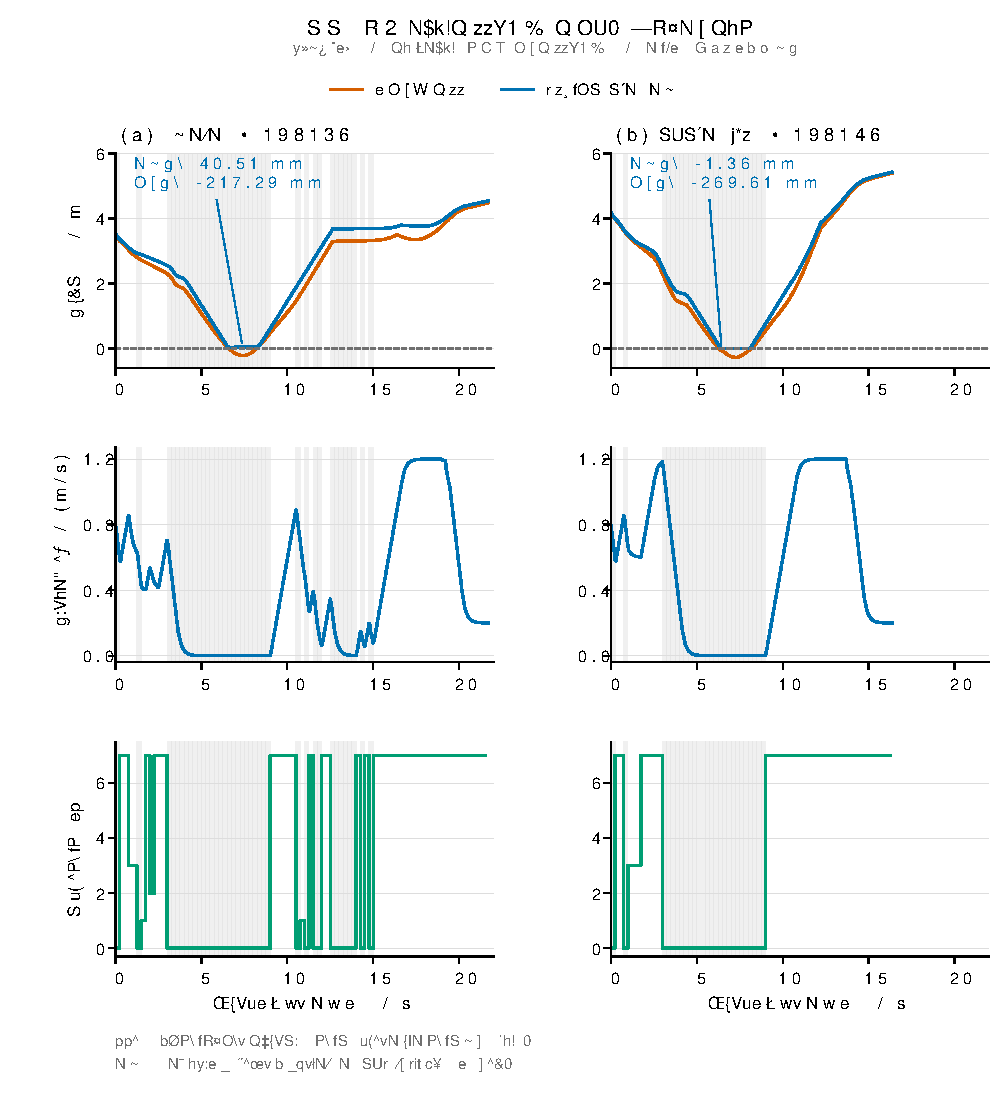
\includegraphics[width=170mm]{H01.pdf}
\caption{图 H01：历史正式研究 R2 中全部两次 PCT 保守净空失败的离线多信号诊断。两列分别为连续交互 seed198136 和单参与者横穿 seed198146。第一行同时绘制原评价器的有裕量圆净空和按记录位姿独立计算的 1.04×0.70 m 车体与 0.72×0.72 m 参与者方盒二维间距；分离时为欧氏最短间距，相交时为负 SAT 最小平移深度。第二行为原日志机器人速度，第三行为每次决策 mask 中可用非停车动作数。灰色区间为执行 action0 的决策周期，并非独立停车事件。两次二维最小值分别为 40.508 mm, -1.361 mm；seed198146 的二维投影相交仅占 1/328 个采样点。原始 contact 计数均为零，历史日志缺少完整 z、roll/pitch 和部件姿态，故不能将投影相交升级为确定物理接触。图为全记录时间线，无平滑、无置信区间，不替代新阶段验证。}
\label{fig:historical-h01}
\end{figure}

\begin{figure}[htbp]
\centering
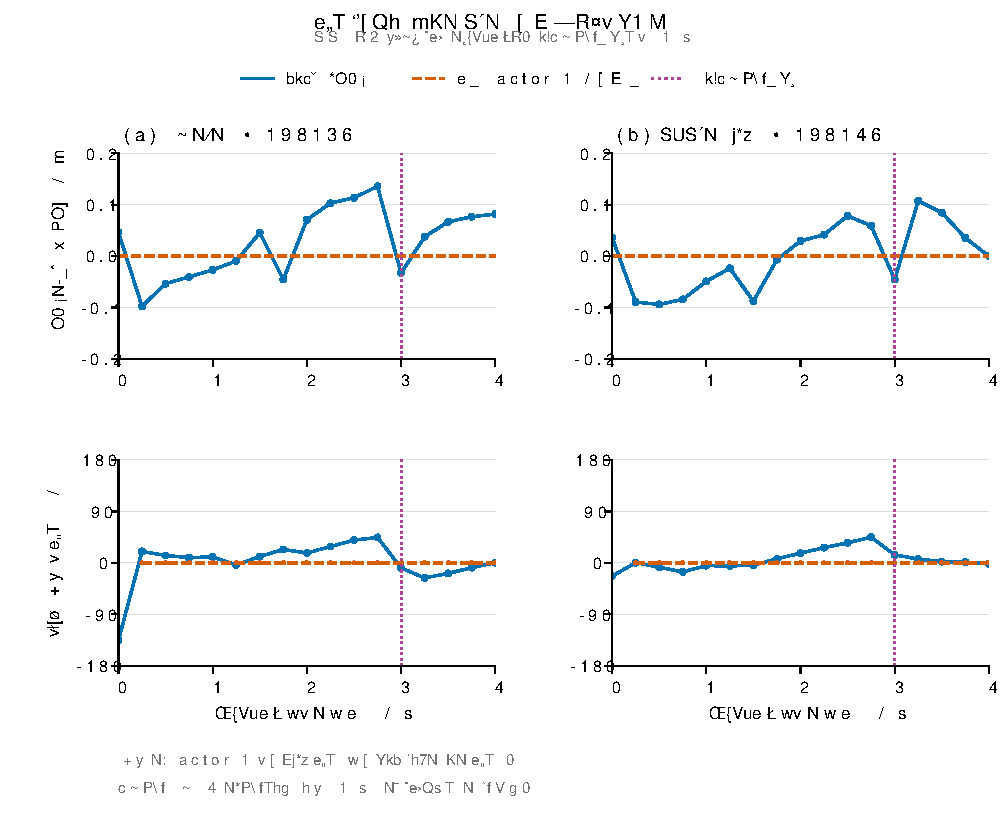
\includegraphics[width=170mm]{H02.pdf}
\caption{图 H02：两次历史 PCT 保守净空失败的扫描跟踪中心与方向诊断。使用同一事件规则：从策略门开始，截取至首次连续四次停车决策开始后的 1 s；完整回合见 H01。上排显示跟踪中心 x 相对日志 actor1 x 的偏差，下排显示安全预测方向与实际 actor1 位移方向相对 +y 的角度；真实位移小于 1 μm 的采样不赋方向角。两例持续停车前最后一次 action3 决策的估计方向分别偏离 +y 44.49° / 44.93°，实际参与者沿 +y 横穿。这些事实支持检验“可见表面中心变化导致方向估计失配”的假设，但不是随机化因果证明；没有重跑旧种子、没有重训或新 Gazebo 样本，曲线不作平滑。}
\label{fig:historical-h02}
\end{figure}

\begin{figure}[htbp]
\centering
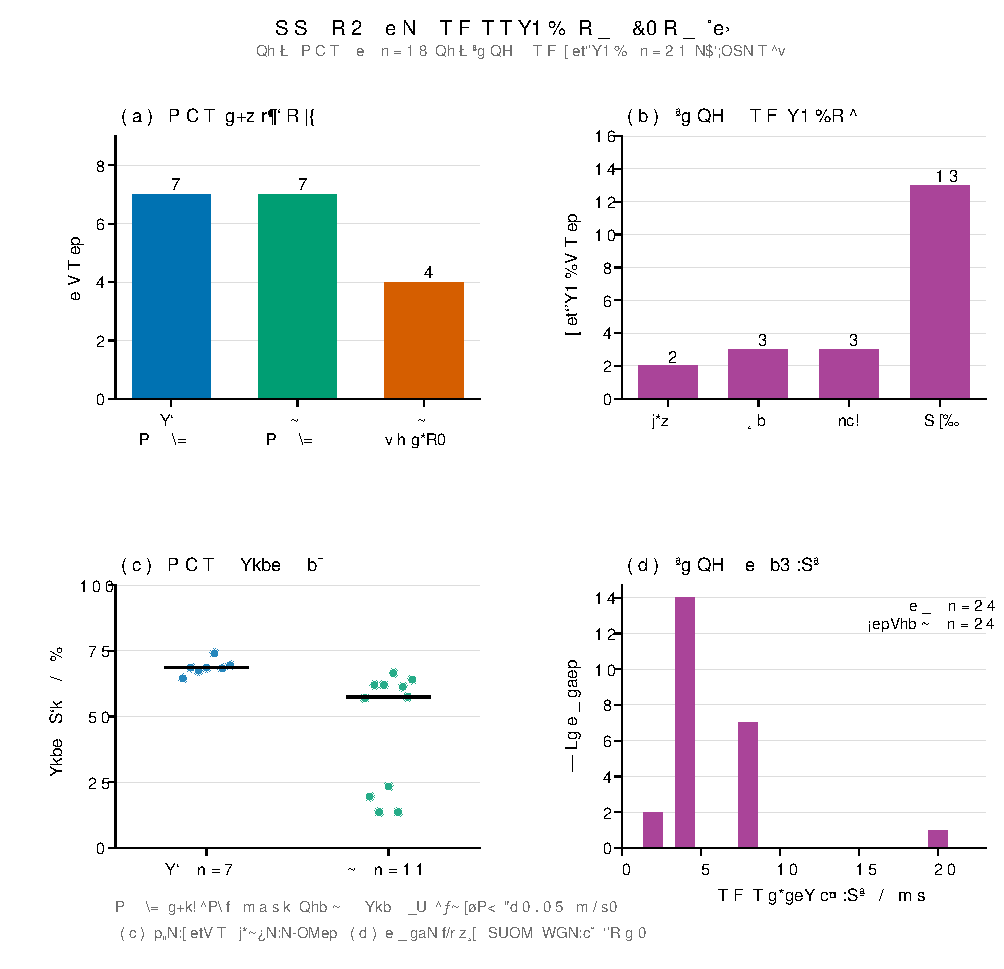
\includegraphics[width=170mm]{H03.pdf}
\caption{图 H03：全部历史 R2 PCT 超时与解析先验 TF 完整性失败的分类诊断。PCT 的 18 次超时按原始末次 mask 与位姿分类：静态：候选耗尽 7 次、连续：候选耗尽 7 次、连续：近目标未到达 4 次。解析先验另有 21 回合违反 scan 时间戳 TF 合同，不能与 PCT 超时合并成一个失败总体。面板(c)以实际记录时间间隔加权计算 |v|≤0.05 m/s 的近静止时长比例，点为完整回合，短横线为组内中位数；不将每次 stop 决策误当独立停车事件。面板(d)仅使用 episode 运行时间内原日志明确报告的向未来外推警告，共 24 条，缺口 2–20 ms；报告计数器累计拒绝 24 个 scan。所有这些 TF 失败回合的最新 TF 查询成功率仍为100%，说明应分别审计最新可用TF与scan采样时刻TF。这些分类支持后继恢复与时间戳队列假设，不构成因果结论或新评估结果；失败均继续保留原22s主指标记账。}
\label{fig:historical-h03}
\end{figure}
